\section{Implementation \& Testing}

This section presents the motivations to implement the MGF-1 function, its implementation and the testing of the the implementation.

\begin{table}[h]
\centering

\begin{adjustbox}{max width=\textwidth}
\begin{tabular}{lccccccccccc}
\hline
	Function  & Total &&  \multicolumn{2}{c@{\hskip 0.2in}}{Polynomial arithmetics} && \multicolumn{2}{c}{Hash functions} && \multicolumn{2}{c}{Rest}\\\cline{4-5}\cline{7-8}\cline{10-11}
 
  & &&$k$ cycles & Percentage && $k$ cycles & Percentage && $k$ cycles & Percentage \\
 \hline
Key genration  & 5424 && 5082 & 93.6\% && 247 & 4.5\% && 95 & 1.7\% \\
Encryption & 1008 && 780 & 77.4\% && 160 & 15.9\% && 68 & 6.7\% \\
Decryption & 1757 && 1560 & 88.8\% & & 104 &5.9\% && 93 & 5.3\%  \\
\hline
\end{tabular}
\end{adjustbox}
\caption{A Cost Breakdown \cite{dai_optimizing_2018} of Reference Code of NTRUEncrypt \cite{noauthor_open_2018}}
\label{tab:cost-breakdown}
\end{table}

The table \ref{tab:cost-breakdown} shows that the hash function takes up to 15.9\% of the total computation cycle number. It is the second most expensive operation after the polynomial arithmetics (that takes up to 93.6\% of the total cycle number). Plus, the rest is negligible as it takes only up to 6.7\%. Hence the hash function $MGF-1$ is a good candidate for performance analysis in order to improve the global computation time by reducing the cycle number. Then, the task to realise was the implementation and optimisation of the $MGF-1$ function in $C$ according to the description of J. Schanck \cite{schanck_practical_2015}. 

\begin{figure}[h]
  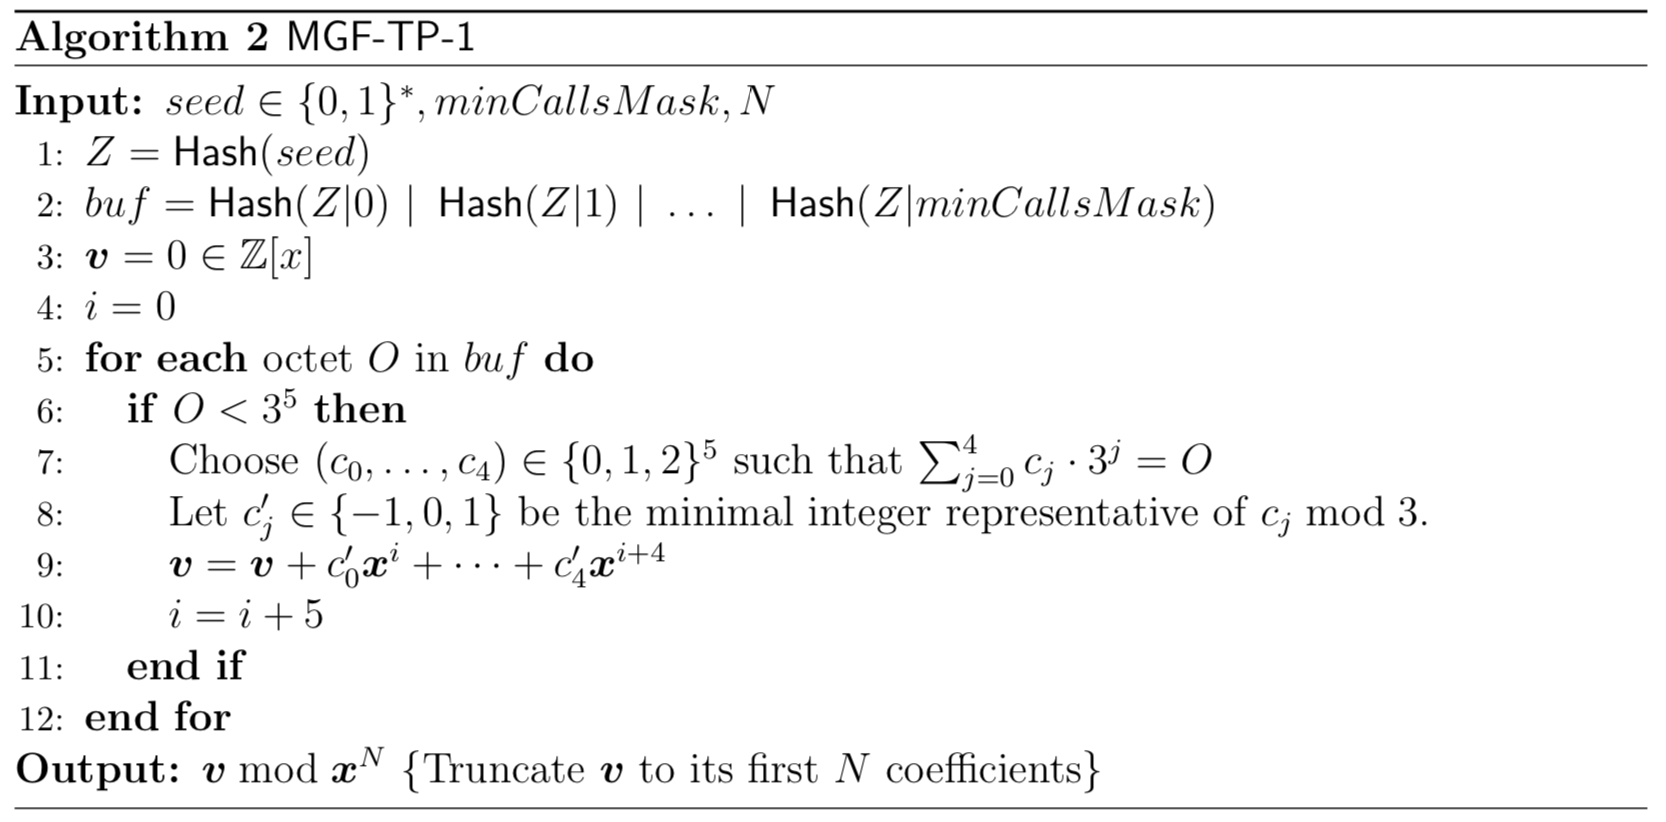
\includegraphics[width=\textwidth]{img/mgf1-description.png}
  \caption{Algorithm MGF-TP-1 \cite{schanck_practical_2015} }
  \label{fig:mgf-1}
\end{figure}

The Figure \ref{fig:mgf-1} shows the description of the algorithm MGF-TP-1 provided by J. Schanck \cite{schanck_practical_2015}. It describes the algorithm from a mathematical point of view. 

The first part of the algorithm (line 1 to 4) calls a hash-function multiple times with different inputs and concatenates the outputs in a $buffer$ to increase the size of the input $seed$.

In the second part (line 5 to 12), it finds a polynomial representation of degree 5 for each bytes of the $buffer$ if the byte is bigger than $3^5$. Else, the byte is dropped to guarantee a uniform distribution of the output. In the description, the polynomial is then formatted to be added to another buffer called $v$.

In the last part, the buffer $v$ is truncated to the $N$ coefficients.

The goal is to implement in a version of the algorithm that will run on an 8-bit AVR Micro-controller. The chosen programming language is C as the code is portable, unlike assembly, and easier to write compare to assembly. Moreover, C allows the programmer to manipulate the memory directly and in efficient way. The performance are typically better with C than other programming languages that require virtual machines like Java. 
% TODO: add that C is used as programming language of the rest of the project and for the reference implementation.
The challenge is to translate this mathematical description of the algorithm into an optimised running version of the algorithm written in C.


As the implementation follows the mathematical description, only the optimisation are described in this section.
The first optimisation is to calculate only the necessary polynomial representations instead of calculating all of them and truncate the result to the first ones. This reduces the computation time, as less computations are necessary. It also reduces the memory usage as it does not store all the polynomial representations. In practice, we don't calculate the polynomial representation of every bytes in the $buffer$ bigger than $3^5$, but only for the $N$ first bytes in the $buffer$ bigger than $3^5$. This implies not calculating $v$ and not performing the modulo operation on $v$. 
The second optimisation is to remove the formatting of line 8. In fact, this formatting is only necessary to compute a correct $v$, which is not required according to the first optimisation.
Moreover, certain memory slot are reused to store different variables to limit the memory usage with the help of pointers in C.
Finally, the compiled assembly code is optimised by Dr. Groszsch\"adl.


This function is implemented following a Test-driven development methodology. Thanks to the already existing implementation of NTRUOpenSourceProject \cite{noauthor_open_2018}, it is possible to compute the output of predefined inputs and therefore to create test cases. The NTRUOpenSourceProject provides a sample execution of the complete NTRU algorithm. However, the NTRUOpenSourceProject does not provide the MGF-1 algorithm as a single C function which makes it harder to determine what correspond to the MGF-1 algorithm, what correspond to its input and output. Using the C debugger on the NTRUOpenSourceProject implementation, it is possible to retrieve the inputs and output of a correct execution of MGF-1 to create the following test case.

\begin{lstlisting}[style=base,frame=single,mathescape=true]
{Test case for MGF-1 implementation}

INPUT 
seed = {0xd0, 0x4c, 0x38, 0xca, 0x20, 0xa1, 0xb5, 0x5f,
	0x3e, 0x95, 0x47, 0x1f, 0x2b, 0xb1, 0xc0, 0x6e,
	0x70, 0xd0, 0xf0, 0x97, 0x52, 0xf4, 0x60, 0x3b,
	0xf5, 0x52, 0xc3, 0x8b, 0x76, 0x7a, 0x32, 0x62,
	0x55, 0x3c, 0xa5, 0xf4, 0x35, 0x06, 0xec, 0xcc,
	0x7d, 0x52, 0x84, 0xe3, 0x3d, 0x24, 0x6e, 0x90,
	0x09, 0xe9, 0xe3, 0xaa, 0x68, 0x71, 0x00, 0x5b,
	0xc8, 0x53, 0x02, 0x80, 0x78, 0xe3, 0x86, 0x2c,
	0xed, 0x91, 0x63, 0x56, 0x5a, 0x3d, 0xc5, 0x7d,
	0xd5, 0x91, 0xaf, 0x9b, 0x96, 0x3c, 0xc7, 0xb5,
	0x6d, 0x5f, 0xe6, 0x6d, 0x8a, 0x06, 0xf5, 0xee,
	0xc6, 0xed, 0xc2, 0x3f, 0x59, 0xb2, 0x07, 0x5f,
	0xb5, 0xb9, 0x60, 0xc7, 0x80}
mincallsMask = 6
N = 20

EXPECTED OUTPUT
mask = {0x00, 0x00, 0x00, 0x01, 0x02, 0x01, 0x00, 0x00, 
	0x02, 0x02, 0x01, 0x01, 0x02, 0x02, 0x00, 0x00,
	0x01, 0x01, 0x00, 0x01}
\end{lstlisting}

This test case is used to determine whether our implementation is correct or not. The implementation and the C version of the test case can be found on the repository of the project \cite{simonetto_ntru_2018}.







